
\section{Placement}
\label{sec:simulated_annealing}
With a basic understanding of FPGA architecture, design placement, and RapidWright, we have all the necessary pieces to implement our SA placer. 
Here we outline in detail each substage of our implementation: PrePacking, Packing, and Placement. 
Shown in Figure \ref{fig:edif_design_device} is an overview of the placement workflow. 
Figure \ref{fig:substages} shows the data structures of RapidWright objects that are populated at each stage. 

{
    \centering
    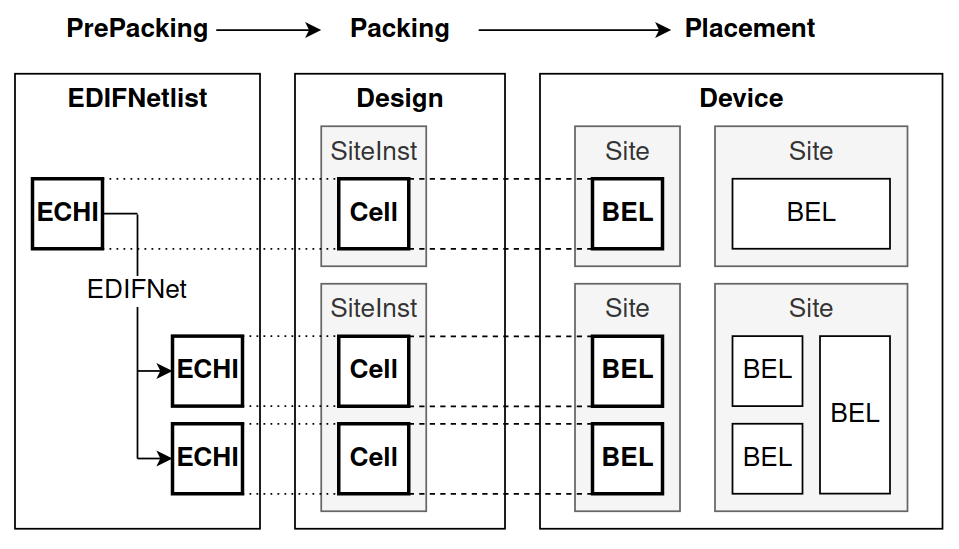
\includegraphics[width=0.9\columnwidth]{figures/edif_design_device.png}
    \captionof{figure}{Our placement workflow}
    \label{fig:edif_design_device}
}

\end{multicols}
{
    \centering
    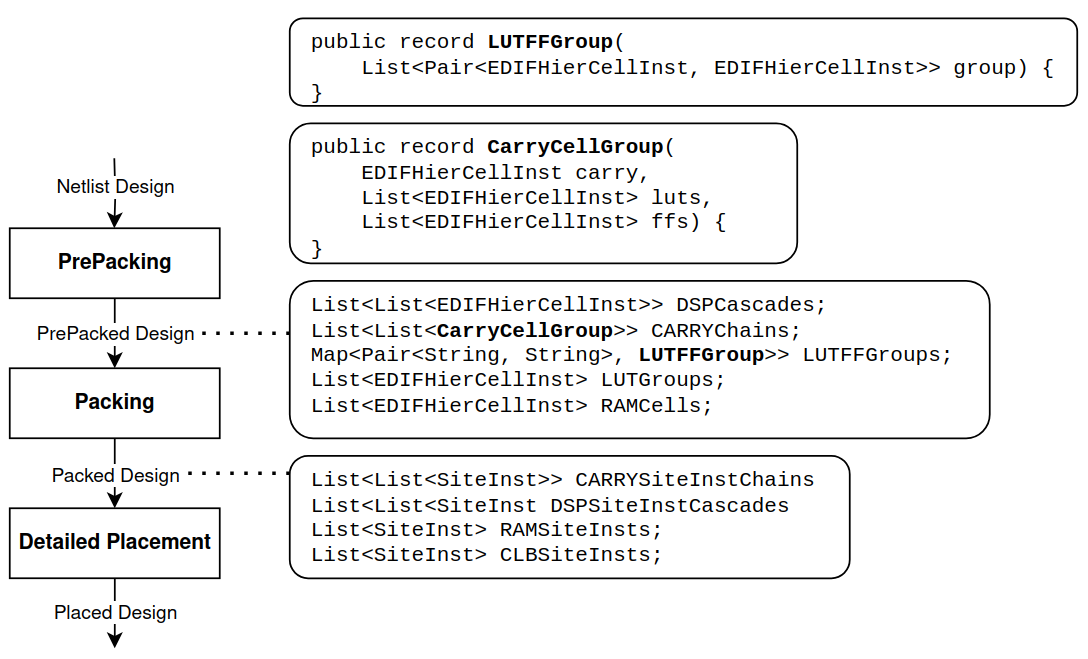
\includegraphics[width=0.8\columnwidth]{figures/substages.png}
    \captionof{figure}{The data classes populated at each substage: PrepackedDesign, PackedDesign, and PlacedDesign.}
    \label{fig:substages}
}
\begin{multicols}{2}

\subsection{Prepacking}
\label{subsec:prepacking}


The first step in our placement flow is \textbf{prepacking}. 
Recall from the 7-Series architecture that there are certain cell structures that must adhere to certain placements constraints to ensure legality, and by design, to minimize wirelength. 
The job of the prepacker is to traverse the raw EDIF netlist, detect these cell structures, and consolidate these cells into clusters or groups of clusters that naturally reflect these placement constraints. 

Recall that CARRY4 chains must necessarily be placed vertically and consecutively across a column of SLICEs in ascending order. 
Likewise, \texttt{DSP48E1} cascades must necessarily be placed vertically and consecutively across a column of DSP48E1 Sites in ascending order. 
A LUT-FF pair may be placed freely, but should be placed in the same lane within the same SLICE to minimize wirelength.

The raw EDIF netlist only tells us the list of nets and the cell ports that they connect to. 
It does not report the presence of any macro cell structures (CARRY4 chains, etc.). 
Thus, we must traverse the netlist to detect these cell structures and store that structure information in a class we will call \texttt{PrepackedDesign}.

A group of LUT-FF pairs may be placed in the same SLICE, with the constraint that the FFs must share the same Clock-Enable (CE) and Set-Reset (SR) nets.
Clustering LUT-FF pairs like this can reduce the redundancy of having to route the same CE and SR nets to many SLICEs by routing the nets to fewer SLICEs and connecting them to the individual FFs within via intra-Site routing, and at the same time, packing greater logic density over a smaller area of the device. 
Recall that up to eight FFs may be placed in the same SLICE, thus theoretically, up to eight LUT-FF pairs can be placed in the same SLICE. 


{
    \centering
    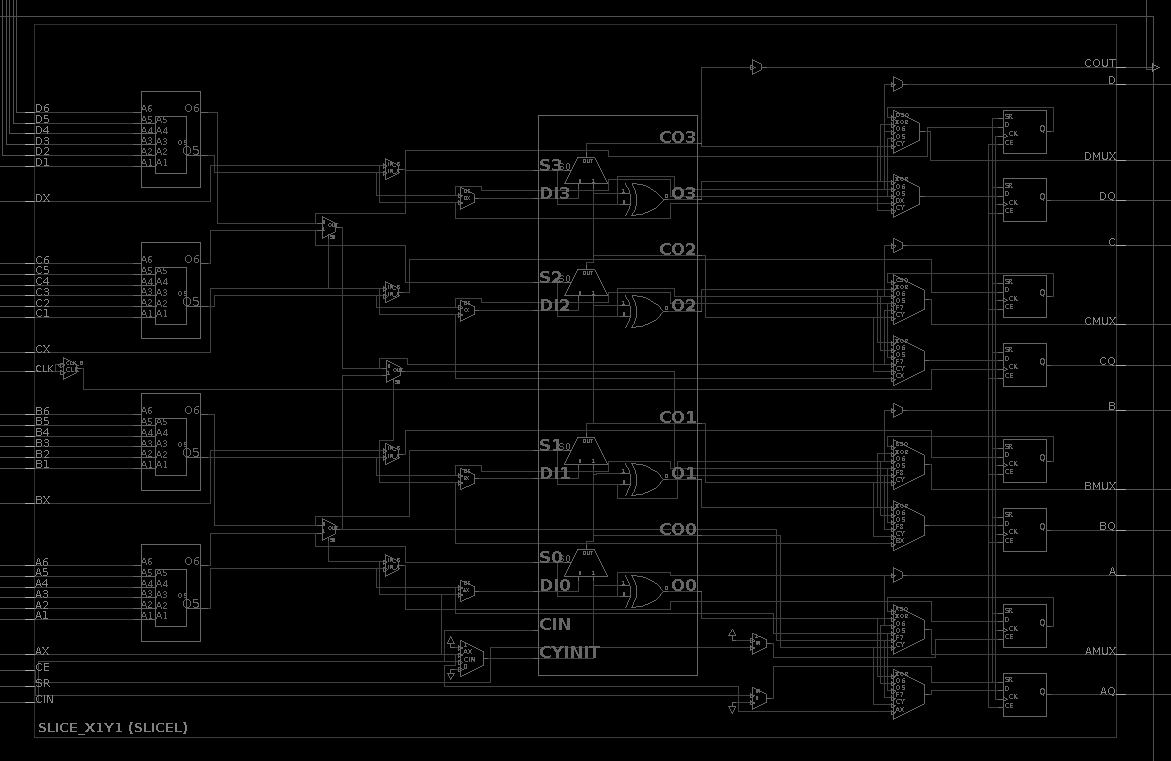
\includegraphics[width=\columnwidth]{figures/slicel.png}
    \captionof{figure}{A SLICEL Site}
    \label{fig:slicel}
}


Utilizing all 8 LUT-FF lanes in a SLICE can help reduce device area utilization and minimize wirelength, but \emph{too much} logic density in an area can contribute to general routing congestion. 
Furthermore, attempting to fill all 8 lanes in a SLICE requires meticulous adherence to conditional LUT constraints. 
Recall that a LUT can accommodate one 6-input boolean function or two 5-input boolean functions sharing the same inputs or any two 3-input or less boolean functions regardless of shared inputs. 
A LUT6 Cell (a LUT with 6-inputs) will actually occupy two LUT-FF lanes in a SLICEL, rendering one of the FF BELs in either lane ineligible for another LUT-FF pair. 
To simplify the problem space, we will only fill up to four LUT-FF lanes in any given SLICE. 


\begin{lstlisting}[language=java, caption={Netlist extraction and traversal}, label={lst:netlist_extract}]
Design design = Design.readCheckpoint("synth.dcp")
EDIFNetlist netlist = design.getNetlist();
List<EDIFCellInst> ecis = netlist.getAllLeafCellInstances();

// Select only the carry cells.
for (EDIFCellInst eci : ecis) {
    if (eci.getCellName() == "CARRY4")
        carryCells.add(eci);
}

// Find and remove carry chains until the list is empty
while (!carryCells.isEmpty()) {
    // Arbitrarily set "currentCell" pointer to a cell in the list
    EDIFCellInst currentCell = carryCells.get(0);

    // Find this carry chain anchor.
    // Traverse the Carry-In (CI) to Carry-Out (CO) nets.
    // Anchor is found when net on the CI Port is Ground.
    while (true) {
        // Access the CI port on this cell.
        EDIFPortInst sinkPort = currentCell.getPortInst("CI");
        // Access the net on this CI port.
        EDIFNet net = sinkPort.getNet();
        if (net.isGND())
            // Found this chain anchor!
            break;
        // Get all ports on this net.
        List<EDIFPortInst> netPorts = net.getPortInsts();
        for (EDIFPortInst netPort : netPorts) {
            // Access the port belonging to another carry cell.
            EDIFCellInst sourceCell = netPort.getCellInst();
            if (sourceCell.getCellName() == "CARRY4") {
                // Move the "currentCell" pointer
                currentCell = sourceCell;
            }
        }
    }

    // Now we have the chain anchor as currentCell.
    // Now traverse in the opposite direction to find the chain tail.
    // Tail is found when the CO Port is null.
    // Collect the chain cells into an ordred list.
    List<EDIFCellInst> currentChain = new ArrayList<>();
    while (true) {
        EDIFPortInst sourcePort = currentCell.getPortInst("CO[3]");
        if (sourcePort == null)
            // Found this chain's tail!
            break;
        EDIFNet net = sourcePort.getNet();
        List<EDIFPortInst> sinkPorts = net.getPortInsts();
        for (EDIFPortInst sinkPort : sinkPorts) {
            EDIFCellInst sinkCell = sinkPort.getCellInst();
            if (sinkCell.getCellName() == "CARRY4") {
                currentCell = sinkCell;
                // Add the cell to the chain list.
                currentChain.add(currentCell);
            }
        }
    }

    // Add currentChain to the list of chains
    carryChains.add(currentChain);
}
\end{lstlisting}


\subsection{Packing}
    \label{subsec:packing}

\subsection{Placement}
    \label{subsec:placement}
    Up until now we have only organized the logical \texttt{Cells} into \texttt{SiteInsts}. 
    This is where simulated annealing actually begins. 

